\documentclass[a4paper]{article}

\usepackage[table]{xcolor}%this has to be the first!!!!!!
\usepackage{fullpage} % Package to use full page
%\usepackage{parskip} % Package to tweak paragraph skipping
\usepackage{tikz} % Package for drawing
\usepackage{tikz-3dplot} % Package for drawing
\usetikzlibrary{shapes,arrows,matrix,positioning,decorations.pathreplacing}

\usepackage{amsmath}
\usepackage{indentfirst}
\usepackage{hyperref}
\usepackage{subcaption}
\usepackage{graphics}
\usepackage{graphicx}
\usepackage{minted}
\usepackage{romannum}
\AtBeginDocument{\pagenumbering{arabic}}% To keep page number arabic

\usepackage{multicol}
\usepackage{mathrsfs}
%color define
\definecolor{codebg}{RGB}{230,255,253}
\definecolor{function}{RGB}{210,0,26}
\definecolor{para}{RGB}{255,137,137}
\definecolor{output}{RGB}{238,224,201}
\setminted[cpp]{mathescape=true,breaklines,bgcolor=codebg,linenos}

\tikzset{
  block/.style = {rectangle, draw, fill=output, text width=6cm, text centered, rounded corners, minimum height=4em},
  line/.style = {draw, -latex'},
}

%function newcommand
\newcommand{\func}[1]{\textbf{\textcolor{function}{#1}}}
\newcommand{\para}[1]{\textbf{\emph{\textcolor{para}{#1}}}}
\newcommand{\activetest}{\tikz \fill[black] (3pt,3pt) circle (3pt);}
\newcommand{\prolong}{\tikz \fill[blue] (3pt,3pt) circle (3pt);}
\newcommand{\rest}{\tikz \fill[red] (3pt,3pt) circle (3pt);}

\usepackage{biblatex}
\addbibresource{bibliography.bib}
\title{heights.h Documentation}
\author{Haochen(Langford) Huang}
\date{\today}

\makeatletter%title setting
\def\@maketitle{%
  \newpage
  \null
  \vskip 2em%
  \begin{center}%
  \let \footnote \thanks
    {\LARGE \@title \par}%
    \vskip 1.5em%
    {\Large
      \lineskip .5em%
      \begin{tabular}[t]{c}%
        \@author
      \end{tabular}\par}%
    \vskip 1em%
    {\large \@date\par}%
    \vskip 1em%
    {\large version: 2.0}%
  \end{center}%
  \par
  \vskip 1.5em}
\makeatother

\begin{document}

\maketitle

\section{Introduction}\label{sec:intro}
'heights.h' together with 'parabola.h' serve as toolbox for 'curvature.h' to compute surface curvature in multiphase flow. The aim of the file is to allocate value which represents distance towards surface to every single cell. And the value is named 'height', therefore the name of current headfile. Before diving into details, I shall first introduce several conceptual definitions with 1D example.
\subsection{Surface}
For each cell, if a 'coherent surface' occurs within certain distance, then the individual will be assigned with valid height value. Otherwise, invalid data 'nodata' will be allocated to such cell. 'coherent surface' defined as process where color function (volume fraction in VOF method) \para{c} changes from $0$ to $1$ or vice versa.

\begin{figure}[h]
  \begin{subfigure}[b]{\textwidth}
     \centering
     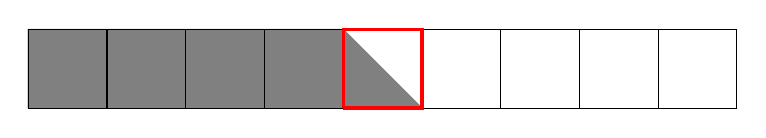
\begin{tikzpicture}[scale=1]
        \filldraw[gray] (-4.0,0)--(1.0,0)--(0,1)--(-4.0,1)--(-4.0,0);
        \draw[step=1cm] (-4.0,0) grid (5.0,1.0);
        \draw[very thick,red] (0,0)--(0,1)--(1,1)--(1,0)--(0,0);
     \end{tikzpicture}
     \subcaption{}
  \end{subfigure}

  \begin{subfigure}[b]{\textwidth}
     \centering
     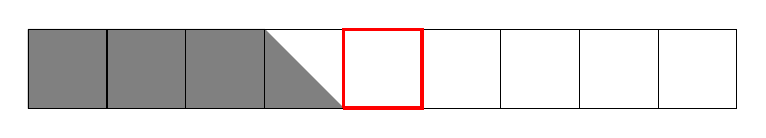
\begin{tikzpicture}[scale=1]
        \filldraw[gray] (-4.0,1)--(-1,1)--(0,0)--(-4.0,0)--(-4.0,1);
        \draw[step=1cm] (-4.0,0) grid (5.0,1.0);
        \draw[very thick,red] (0,0)--(0,1)--(1,1)--(1,0)--(0,0);
     \end{tikzpicture}
     \subcaption{}
  \end{subfigure}

  \begin{subfigure}[b]{\textwidth}
     \centering
     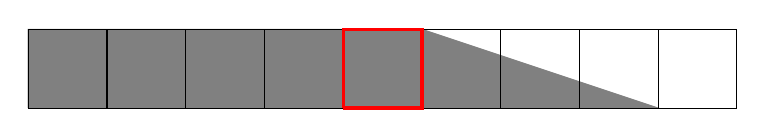
\begin{tikzpicture}[scale=1]
        \filldraw[gray] (-4.0,0)--(4.0,0)--(1.0,1)--(-4.0,1)--(-4.0,0);
        \draw[step=1cm] (-4.0,0) grid (5.0,1.0);
        \draw[very thick,red] (0,0)--(0,1)--(1,1)--(1,0)--(0,0);
     \end{tikzpicture}
     \subcaption{}
  \end{subfigure}
  \caption{Graphical representation of coherent surface. Cell highlighted by red square represents current cell. Color grey indicates volume fraction.}
  \label{fig:surface}
\end{figure}
Figure \ref{fig:surface} displays occasions where height value is valid for current cell (the one hightlighted by red square). Within certain distance, cell fully immersed in color function (represents by color grey) and those with $0$ value both occur. On the contrary, figure \ref{fig:nosurface} demonstrates occasions in which 'coherent surface' is not observed. Therefore 'nodata' is assigned.
\begin{figure}
  \begin{subfigure}[b]{\textwidth}
     \centering
     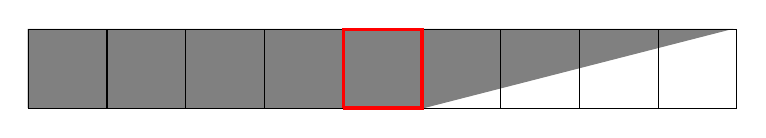
\begin{tikzpicture}[scale=1]
        \filldraw[gray] (-4.0,0)--(1.0,0)--(4.9,1)--(-4.0,1)--(-4.0,0);
        \draw[step=1cm] (-4.0,0) grid (5.0,1.0);
        \draw[very thick,red] (0,0)--(0,1)--(1,1)--(1,0)--(0,0);
     \end{tikzpicture}
     \subcaption{}
  \end{subfigure}

  \begin{subfigure}[b]{\textwidth}
     \centering
     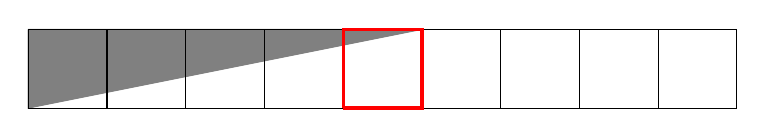
\begin{tikzpicture}[scale=1]
        \filldraw[gray] (-4.0,1)--(1,1)--(-4,0)--(-4.0,1);
        \draw[step=1cm] (-4.0,0) grid (5,1.0);
        \draw[very thick,red] (0,0)--(0,1)--(1,1)--(1,0)--(0,0);
     \end{tikzpicture}
     \subcaption{}
  \end{subfigure}

 \begin{subfigure}[b]{\textwidth}
     \centering
     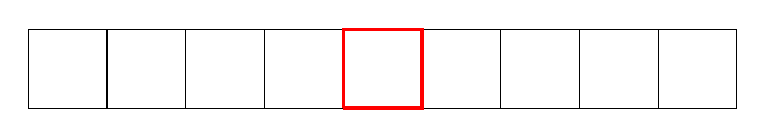
\begin{tikzpicture}[scale=1]
        \draw[step=1cm] (-4.0,0) grid (5,1.0);
        \draw[very thick,red] (0,0)--(0,1)--(1,1)--(1,0)--(0,0);
     \end{tikzpicture}
     \subcaption{}
  \end{subfigure}
  \caption{Graphical representation of not coherent surface. Cell highlighted by red square represents current cell. Color grey indicates volume fraction.}
  \label{fig:nosurface}
\end{figure}

\subsection{Height value and 0 value point}
Nature of height value is the summary of color function, and the value of each cell is represented by that at center of the individual. In order to obtain specific value, the position where $0$ is located should first be defined.
Consider a condition as illustrated in figure \ref{fig:0position} where surface is indeed two cell with color function of $0.6$ and $0.1$. 0 point then located at the place $0.7$ away from the final occupied cell i.e. blue line in figure \ref{fig:0position}. Then value of each cell is calculated based on the distance between cell center and 0 position as demonstrated beneath the figure. The positive direction points towards inner side of surface.
\begin{figure}
    \centering
    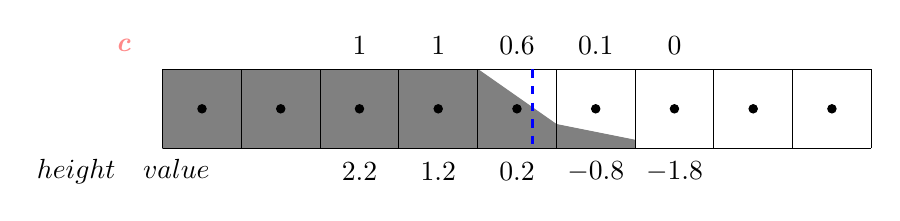
\begin{tikzpicture}[scale=1]
        \filldraw[gray] (-4.0,1)--(0,1)--(0,0)--(-4,0)--(-4.0,1);
        \filldraw[gray] (0.0,1)--(0,0)--(1,0)--(1,0.3)--(0,1);
        \filldraw[gray] (1.0,0.3)--(2,0.1)--(2,0)--(1,0)--(1,0.3);
        \draw[step=1cm] (-4.0,0) grid (5,1.0);
        \node at (-4.5,1.3) {\para{c}};
        \node at (0.5,1.3) {$0.6$};
        \node at (-0.5,1.3) {$1$};
        \node at (1.5,1.3) {$0.1$};
        \node at (-1.5,1.3) {$1$};
        \node at (2.5,1.3) {$0$};
        
        \node at (-4.5,-0.3) {$height\quad value$};
        \node at (0.5,-0.3) {$0.2$};
        \node at (-0.5,-0.3) {$1.2$};
        \node at (1.5,-0.3) {$-0.8$}; 
        \node at (-1.5,-0.3) {$2.2$};
        \node at (2.5,-0.3) {$-1.8$};
        \draw[very thick,dashed,blue](0.7,1)--(0.7,0);

        \foreach \x in {-3.5,-2.5,...,4.5}
        {
          \filldraw[] (\x,0.5) circle (1.5pt);
        }
    \end{tikzpicture}
    \caption{Graphical representation of 0 position. Blue dashed line indicates the exact position of 0 position. Numbers on the top reveals the color function of each cell while those beneath displays corresponding height value at center of each cell as shown by black dot.}
    \label{fig:0position}
\end{figure}
\subsection{Direction of surface}
Except example shown in figure \ref{fig:0position} there do exist another possibility that surface stems following opposite direction (from right to left in this example). In order to distinguish these two occasions the value of 0 position is defined to be 20 for cases show in figure \ref{fig:direction}. Typically, only cells positioned within $5.5$ distance away from 0 position has valid height value. Therefore the range of height value is $[-5,5]$ or $[15,25]$ based on surface direction.

\begin{figure}
    \centering
    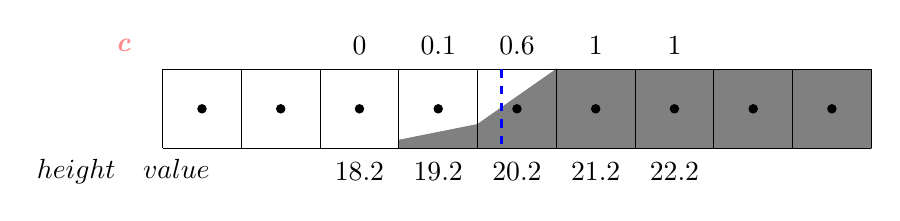
\begin{tikzpicture}[scale=1]
        \filldraw[gray] (1.0,1)--(1,0)--(5,0)--(5,1)--(1.0,1);
        \filldraw[gray] (1.0,1)--(1,0)--(0,0)--(0,0.3)--cycle;
        \filldraw[gray] (0.0,0.3)--(-1,0.1)--(-1,0)--(0,0)--(0,0.3);
        \draw[step=1cm] (-4.0,0) grid (5,1.0);
        \node at (-4.5,1.3) {\para{c}};
        \node at (0.5,1.3) {$0.6$};
        \node at (-0.5,1.3) {$0.1$};
        \node at (1.5,1.3) {$1$};
        \node at (-1.5,1.3) {$0$};
        \node at (2.5,1.3) {$1$};
        
        \node at (-4.5,-0.3) {$height\quad value$};
        \node at (0.5,-0.3) {$20.2$};
        \node at (-0.5,-0.3) {$19.2$};
        \node at (1.5,-0.3) {$21.2$}; 
        \node at (-1.5,-0.3) {$18.2$};
        \node at (2.5,-0.3) {$22.2$};
        \draw[very thick,dashed,blue](0.3,1)--(0.3,0);

        \foreach \x in {-3.5,-2.5,...,4.5}
        {
          \filldraw[] (\x,0.5) circle (1.5pt);
        }
    \end{tikzpicture}
    \caption{Graphical representation of 0 position. Blue dashed line indicates the exact position of 0 position. Numbers on the top reveals the color function of each cell while those beneath displays corresponding height value at center of each cell as shown by black dot.}
    \label{fig:direction}
\end{figure}

\section{Functions}\label{sec:funcc}
\subsection{Overall configuration}\label{sec:config}
Before introducing parameters and workflow, I shall firstly deliver a brief introduction about overall configuration of three functions which will be discussed in the following sections. Figure \ref{fig:funcconfig} depicts the overall function configuration of current headfile. \func{heights} serves as console and delivers command to \func{half\_column} in which volume fraction integration is conducted on neighbourhood cells. After iterating the adjoining $8$ cells (4 for both positive and negative direction), the height value is allocated to the current cell. Note that special care is taken for tree girds and the additional function \func{refine\_h\_x} is employed to prolongate color function on tree grid.  
\begin{figure}
    \centering
    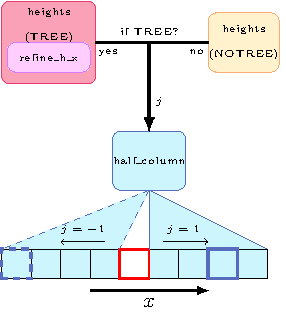
\includegraphics[width=0.6\textwidth]{image/heights.pdf}
    \caption{Overall configuration of current headfile. Red square highlights current cell and the blue square represents cell scanned by \func{half\_column}.}
    \label{fig:funcconfig}
\end{figure}
\subsection{\func{height}\&\func{orientation}}
\subsubsection{Worth mentioning details}
These two functions are 'tricky' functions. As introduced in section \ref{sec:intro}, in order to distinguish the orientation of the surface, range of final value has two options: $[-5,5]$ or $[15,25]$. \func{height} is the reverse function which takes height value as input, erases disguise of orientation and returns the real distance between current cell and 0 position. The range of corresponding output turns out to be $[-10,10]$.\par
By contrary \func{orientation} returns surface orientation based on height value. To save memory, tricky function manifests as 'inline' function, i.e. substitute corresponding code when it is called.
\subsubsection{Workflow}
\begin{multicols}{2}
  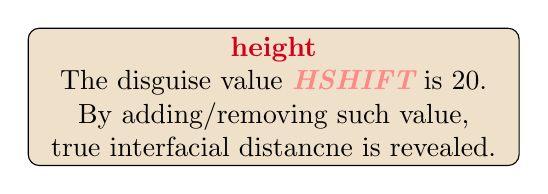
\begin{tikzpicture}
    \node [block]{
        \func{height}\\
        The disguise value \para{HSHIFT} is $20$. By adding/removing such value, true interfacial distancne is revealed. 
      };
  \end{tikzpicture}
 \columnbreak
 \begin{minted}{cpp}
#define HSHIFT 20.

static inline double height (double H) {
  return H > HSHIFT/2. ? H - HSHIFT : H < -HSHIFT/2. ? H + HSHIFT : H;
}
 \end{minted}
\end{multicols}

\begin{multicols}{2}
  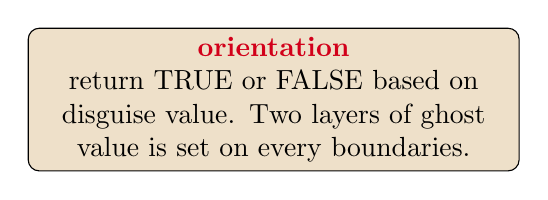
\begin{tikzpicture}
    \node [block]{
        \func{orientation}\\
        return TRUE or FALSE based on disguise value. Two layers of ghost value is set on every boundaries.
      };
  \end{tikzpicture}
 \columnbreak
 \begin{minted}{cpp}
static inline int orientation (double H) {
  return fabs(H) > HSHIFT/2.;
}

#define BGHOSTS 2
 \end{minted}
\end{multicols}
\subsection{\func{half\_column}}
Based on previous discussion \func{half\_column} plays major role in height computing whose duty is to scan over neighborhood cells and feedback status value of surface finding as well as height value. Owing to its complexity, I shall carefully interpret the algorithm part by part instead of briefly introducing selected details.
\subsubsection{Parameters}
\begin{center}
  \begin{tabular}{|c|c|c|c|c|}
    \hline
    Name & Data type & Status & Option/Default & Representation (before/after)\\[0.5ex]
    \hline\hline
    \para{point} & Point & unchanged & compulsory & current cell position\\
    \hline
    \para{c} & scalar & unchanged & compulsory & $ c $ (volume fraction)\\
    \hline
    \rowcolor{output}\para{h} & vector & \textbf{output} & compulsory & $\mathbf{h}$\\
    \hline
    \para{cs} & scalar & unchanged & compulsory & $c[2*j]$\\
    \hline
    \para{j} & int & unchanged & compulsory & $j$ (direction control)\\
    \hline
  \end{tabular}
\end{center}

\subsubsection{Purpose of the function}\label{sec:purpose}
\func{half\_column} has two purposes:
\begin{enumerate}
    \item To check whether there is a coherent surface (defined in section \ref{sec:intro}) within 8 adjoining cells.
    \item If there is coherent surface, compute corresponding height value by integrating color function of each cell.
\end{enumerate}
There are three possible situations for current cell: $f_c=1,f_c=0,f_c\in(0,1)$. Where $f_c$ represents color function value of current cell. For first two situations, the threshold for coherent surface is to find certain neighborhood in which $f=0,f=1$ respectively. However for third condition i.e. the cell located on surface, one should iterate both directions to find a pair of opposite (full and empty) cells on each side.\par
\begin{figure}
    \centering
    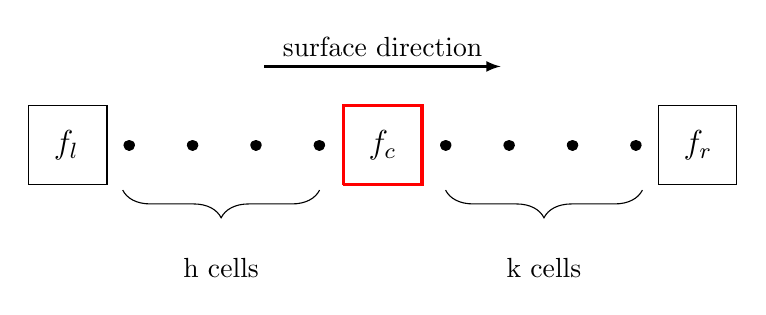
\begin{tikzpicture}[scale=1,circle dotted/.style={dash pattern=on .05mm off 8mm,line cap=round}]
        \draw (0-4,0)--(0-4,1)--(1-4,1)--(1-4,0)--(0-4,0);
        \draw[very thick,red] (0,0)--(0,1)--(1,1)--(1,0)--(0,0);
        \draw (0+4,0)--(0+4,1)--(1+4,1)--(1+4,0)--(0+4,0);
        \draw[line width = 4,circle dotted] (1.3,0.5) -- (3.8,0.5);
        \draw[line width = 4,circle dotted] (-0.3,0.5) -- (-2.8,0.5);
        \draw[decorate,decoration={brace,amplitude=10,mirror,raise=2}] (1.3,0) --(3.8,0) node[midway,yshift=-3em] {k cells};
        \draw[decorate,decoration={brace,amplitude=10,raise=2}] (-0.3,0) --(-2.8,0) node[midway,yshift=-3em] {h cells};
        \node[anchor=west] at (0.2,0.5) {\large$f_c$};
        \node[anchor=west] at (4.2,0.5) {\large$f_r$};
        \node[anchor=west] at (-3.8,0.5) {\large$f_l$};
        \draw[thick,-latex] (-1,1.5)--(2,1.5) node[above,midway] {surface direction};
    \end{tikzpicture}
    \caption{Sketch of position switching between cells. $f_c,f_r,f_l$ represent color function value of current cell (red square) and its right/left side neighbor, respectively.}
    \label{fig:possw}
\end{figure}
Once coherent surface is found, the problem remaining is how to calculate the height value. The key to understand such process is position switch between cells. Figure \ref{fig:possw} displays an example of such condition, where $f_c,f_r,f_l$ represent color function value of corresponding cell. Following the surface direction (defined as vetor points from inner side to outside of surface, e.g. figure \ref{fig:0position}.), relationship between three values reads
\begin{align}
    f_c-(k+1)=f_r\\
    f_c+(h+1)=f_l
\end{align}
Among all the cells, the one whose height value is easiest to obtain is the final full cell close to the surface (hereinafter as final cell). Figure \ref{fig:hvcomp} demonstrates same example in figure \ref{fig:0position} but highlight the final cell and corresponding surface direction. Based on discussion in section \ref{sec:intro}, the height value of final cell can be compute by integrating the color function along surface direction till the very first empty one (cell $E$) reads:
\begin{equation}
    h_B=h_B+h_C+h_D+h_E-0.5=1+0.6+0.1+0-0.5=1.2
\end{equation}
Three terms in R.H.S represents color function of cell $B,C,D,E$.
While the $-0.5$ stems from the fact that height value of one cell is determined from its center instead of left boundary. Combined with the position switch discussed previously, we can then obtain height value of every cell. In short, to obtain a height value, one should first switch to 'final cell' and integrate through surface. For example, height value of cell $F$ yields $h_F=h_B-4=-2.8$ and that of cell $A$ yields $h_A=h_B+1=2.2$.
\begin{figure}
    \centering
    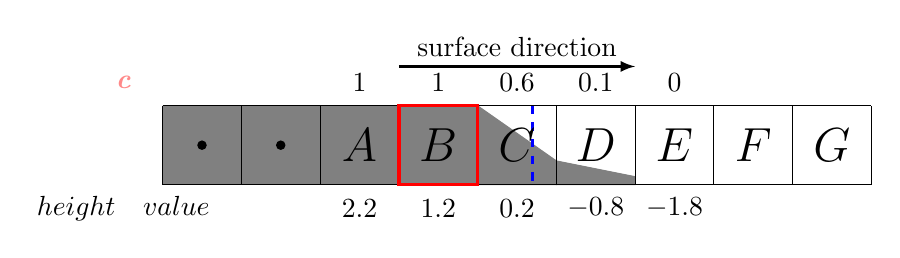
\begin{tikzpicture}[scale=1]
        \filldraw[gray] (-4.0,1)--(0,1)--(0,0)--(-4,0)--(-4.0,1);
        \filldraw[gray] (0.0,1)--(0,0)--(1,0)--(1,0.3)--(0,1);
        \filldraw[gray] (1.0,0.3)--(2,0.1)--(2,0)--(1,0)--(1,0.3);
        \draw[step=1cm] (-4.0,0) grid (5,1.0);
        \node at (-4.5,1.3) {\para{c}};
        \node at (0.5,1.3) {$0.6$};
        \node at (-0.5,1.3) {$1$};
        \node at (1.5,1.3) {$0.1$};
        \node at (-1.5,1.3) {$1$};
        \node at (2.5,1.3) {$0$};
        
        \node at (-4.5,-0.3) {$height\quad value$};
        \node at (0.5,-0.3) {$0.2$};
        \node at (-0.5,-0.3) {$1.2$};
        \node at (1.5,-0.3) {$-0.8$}; 
        \node at (-1.5,-0.3) {$2.2$};
        \node at (2.5,-0.3) {$-1.8$};
        \draw[very thick,dashed,blue](0.7,1)--(0.7,0);

        \draw[very thick, red](-1,0)--(-1,1)--(0,1)--(0,0)--cycle;

        \foreach \x in {-3.5,-2.5}
        {
          \filldraw[] (\x,0.5) circle (1.5pt);
        }

        \node at (-1.5,0.5) {\LARGE$A$};
        \node at (-0.5,0.5) {\LARGE$B$};
        \node at (0.5,0.5) {\LARGE$C$};
        \node at (1.5,0.5) {\LARGE$D$};
        \node at (2.5,0.5) {\LARGE$E$};
        \node at (3.5,0.5) {\LARGE$F$};
        \node at (4.5,0.5) {\LARGE$G$};

        \draw[thick,-latex] (-1,1.5)--(2,1.5) node[above,midway] {surface direction};
    \end{tikzpicture}
    \caption{Same example as in figure \ref{fig:0position} with two example stencils $A,B$. Red square here used to highlight the final full cell next to surface.}
    \label{fig:hvcomp}
\end{figure}
\subsubsection{Configuration of the function}
Figure \ref{fig:column} carefully depicts configuration of \func{half\_column} which consists of three layer. As illustrated in figure \ref{fig:funcconfig} and section \ref{sec:funcc}, \func{half\_column} will be called twice during the process, first for negative direction $(j=-1)$ then for positive direction $(j=1)$. Except for second layer 'iteration', the rest two will be altered according to direction.\par
Parameter \para{S} is employed to record status of process: if a current surface is found then the height function is complete (\para{S}=-1) or one end is found (\para{S}=1 or \para{S}=0) or no end is found (\para{S}$\in (0,1)$). Note that \para{S} is defined within \func{half\_column} and thus will be cleared once function ends therefore a method is needed to preserve results of negative direction. Basilisk achieve such goal by encoding status along with current height result \para{H} into \para{h[]} and decode such value to restore at beginning of second cycle when $j=1$.\par
Coming back to the overall process, the decode step, if needed, is carried out along with initial settings in the first layer. After which height value is calculated and stored as \para{H} in the second layer 'iteration' by checking neighborhood cells. \para{S} is also altered with respect to the iterating results. \para{h[]} which serves as output is processed in the final layer. Depending on 
the direction, it will be encoded or directly output. Careful introductions are presented in the following sections.
\subsubsection{first layer}
There are three possible occasions for \para{S} as initial status obtained from volume fraction of current cell (highlighted by red square), i.e. $0,1,f$ corresponds to empty, full and surface cell. If is in the second cycle $(j=1)$, an additional step is carried out to decode \para{h[]} from which status and height value obtained in previous cycle can be restored in \para{stats.s} and \para{stats.h} respectively.\par
There are totally four occasions which will be encountered in decoding process:
\begin{enumerate}
    \item $\para{h[]}=300,(\para{stat.s},\para{stat.h})=(-1,nodata)$: Those whose current cell is not surface cell ($\para{c[]}=1\ or\ 0$) and fails to find coherent surface, or current cell is surface cell and fails to find empty/full cell during first cycle.
    \item $90\leq\para{h[]}<190,(\para{stat.s},\para{stat.h})=(0,\para{h[]}-100)$: Current cell is surface cell and find empty cell during first cycle.
    \item $190\leq\para{h[]},(\para{stat.s},\para{stat.h})=(-1,h[]-200)$: Current cell is surface cell and find full cell during first cycle.
    \item $-10\leq\para{h[]}<90,(\para{stat.s},\para{stat.h})=(-1,h[])$: Current cell is empty/full cell and find coherent surface during first cycle.    
\end{enumerate}
For occasion 2 and 3, \para{S} and \para{H} are assigned with \para{stats.s} and \para{stats.h} and continue its journey on finding another end to accomplish a coherent surface. Otherwise \para{S} and \para{H} preserve to be the outcome of initial.
\subsubsection{second layer}
As depicted in figure \ref{fig:column}, there are overall 5 categories of occasions and lead to 4 kinds of results. Note all those occasions stem from three types of \para{S} instead of volume fraction of current cell.
\begin{itemize}
    \item[A] $0<\para{S}=f<1$: Find empty/full cell, \para{S} switch to $0/1$ and results in condition \Romannum{1}/\Romannum{2} respectively. One end of coherent surface has been found.
    \item[B] $\para{S}=1$: Find empty cell which indicates occurrence of coherent surface. \para{S} switch to $-1$, the iteration completes and leads to condition \Romannum{3}.
    \item[C] $\para{S}=0$: Find full cell which indicates occurrence of coherent surface. \para{S} switch to $-1$, the iteration completes and leads to condition \Romannum{3}.
    \item[D] $\para{S}=1\ or\ \para{S}=0$: Scan over a surface cell then returning to the one with the same status as \para{S}. Consider the program is set to scan over only four neighborhood cells, such occasion suggests failure of finding coherent surface on this direction. Indeed, such filter is set to tackle situation demonstrated in figure \ref{fig:Dtarget}. This leads to condition \Romannum{4} and \para{S} keeps unchanged.
    \item[others]: Except occasions have been mentioned, the rest all fail to find coherent surface or at least one end of it (for surface cell). These occasions do not change \para{S} and leads to condition \Romannum{4}.
\end{itemize}
\begin{figure}
    \centering
    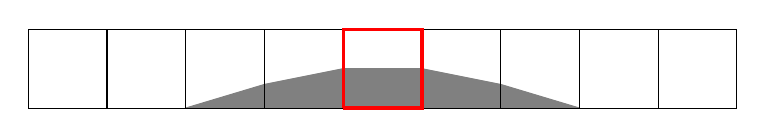
\begin{tikzpicture}[scale=1]
        \filldraw[gray] (-2,0)--(-1,0.3)--(0,0.5)--(1,0.5)--(2,0.3)--(3,0);
        \draw[step=1cm] (-4.0,0) grid (5,1.0);
        \draw[very thick,red] (0,0)--(0,1)--(1,1)--(1,0)--(0,0);
    \end{tikzpicture}
    \caption{The situation that the second layer occasion D aims to tackle.}
    \label{fig:Dtarget}
\end{figure}
The accumulation of height value is carried out in this layer but expresses implicitly in figure \ref{fig:column}. Following the protocol introduced in section \ref{sec:purpose}, the height value is first output and added by $\para{HSHIFT}=20$ if surface direction is against coordinate, as discussed in section \ref{sec:config}.
\subsubsection{third layer}\label{sec:thirdl}
If direction is negative ($j=-1$), the output status along with height value will be encode into \para{h[]} in this layer. Four kinds of conditions output by second layer will be divided into three kinds of categories.
\begin{itemize}
    \item[A] condition \Romannum{4}, height value is encoded as $\para{h[]}=300$: The cases that fail to find coherent surface marked as 'inconsistent'.
    \item[B] condition \Romannum{3}, height value is not encoded $\para{h[]}=\para{H}$: Those cases successfully find coherent surface.
    \item[C] condition \Romannum{1} and \Romannum{2}, height value is encoded as \Romannum{1}: $\para{h[]}=\para{H}+100$, \Romannum{2}: $\para{h[]}=\para{H}+200$: Cases whose current cell is surface cell and find empty/full cell as one end of coherent surface.
\end{itemize}
If direction is positive ($j=1$) the third layer then acts as the final output. Before finally assigning \para{h[]}, two occasions 
\begin{enumerate}
    \item condition \Romannum{5}: Surface cell as current cell and find one end during first cycle.
    \item condition \Romannum{3}: coherent surface is found in second cycle and height value in second cycle appears less than the previous cycle i.e. $\para{H}<\para{stats.h}$.
\end{enumerate}
update data as $(\para{stats.s},\para{stats.h})=(\para{S},\para{H})$. The second occasion indicates when single cell obtains two valid height value, the less one will be admitted. 
Since \para{nodata} defined in Basilisk is an extreme large integer, occasion 2 also covers situations which fails to find coherent surface in first cycle but succeed in the second cycle.\par
Final height value $\para{h[]}$ therefore assigned according to $(\para{stats.s},\para{stats.h})$ as shown in figure \ref{fig:column}.
\begin{figure}
    \centering
    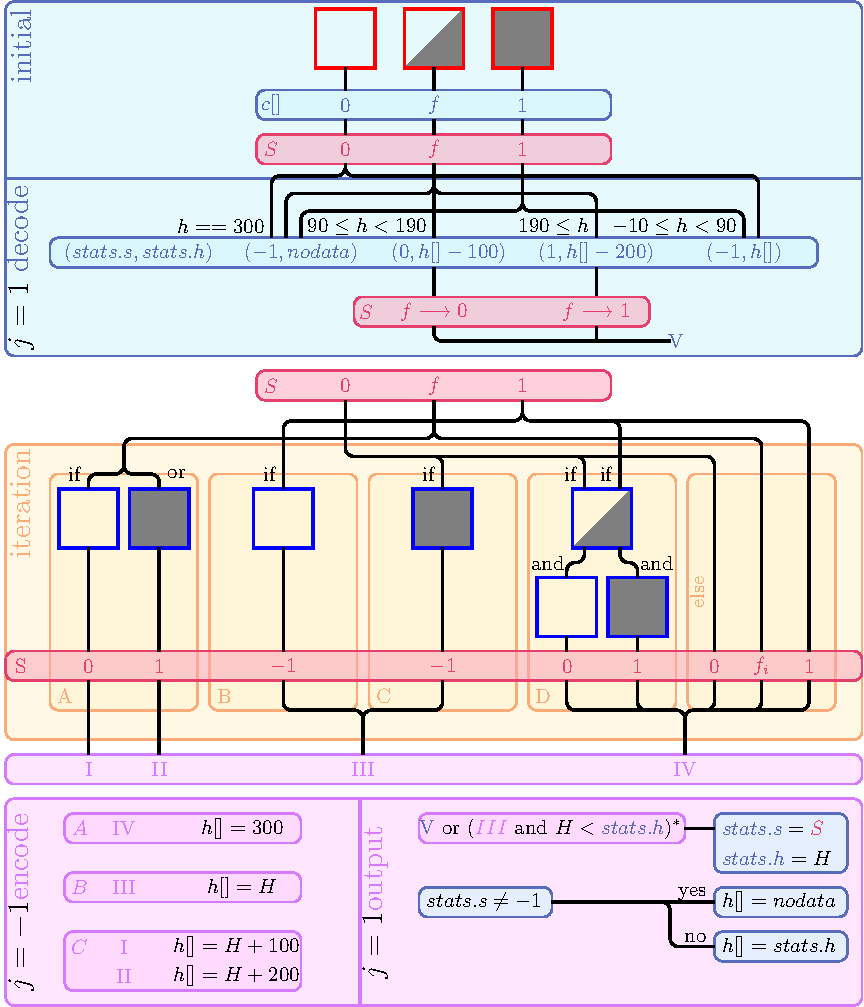
\includegraphics[width=\textwidth]{image/column.pdf}
    \caption{Detailed description about \func{half\_column}. For sake of simplicity, some tricky treats have been hidden. For instance judgement in third layer highlighted by $\ast$ compares surface distance instead of direct value of $H$ and $stats.h$. Therefore the actual form of judgement reads $fabs(height(H))<fabs(height(stats.h))$.}
    \label{fig:column}
\end{figure}
\newpage
\subsubsection{Program Workflow}
\begin{multicols}{2}
  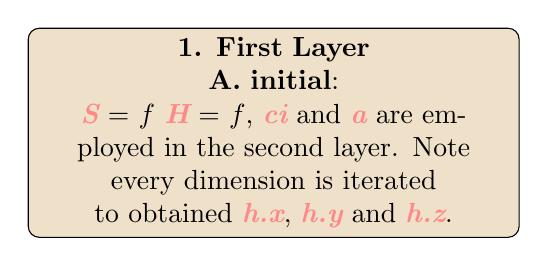
\begin{tikzpicture}
    \node [block]{
        \textbf{1. First Layer}\\
        \textbf{A. initial}:\\
        \para{S} = $f$ \para{H} = $f$, \para{ci} and \para{a} are employed in the second layer. Note every dimension is iterated to obtained \para{h.x}, \para{h.y} and \para{h.z}.
      };
  \end{tikzpicture}
 \columnbreak
 \begin{minted}{cpp}
static void half_column (Point point, scalar c, vector h, vector cs, int j)
{
  const int complete = -1;
  foreach_dimension() {
    double S = c[], H = S, ci, a;
 \end{minted}
 
\end{multicols}

\begin{center}
  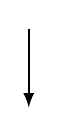
\begin{tikzpicture}
    \draw[-latex,thick](0,0) -- (0,-1); 
  \end{tikzpicture}
\end{center}

\begin{multicols}{2}
  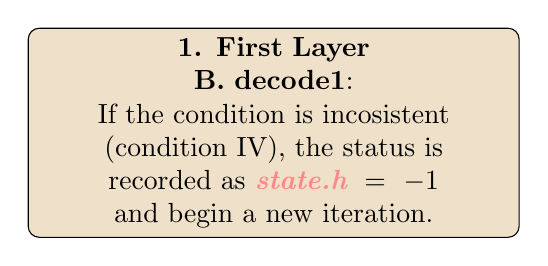
\begin{tikzpicture}
    \node [block]{
        \textbf{1. First Layer}\\
        \textbf{B. decode1}:\\
        If the condition is incosistent (condition \Romannum{4}), the status is recorded as $\para{state.h}=-1$ and begin a new iteration.
      };
  \end{tikzpicture}
 \columnbreak
 \begin{minted}{cpp}
    typedef struct { int s; double h; } HState;
    HState state = {0, 0};
    if (j == 1) {

      if (h.x[] == 300.)
	state.s = complete, state.h = nodata;
 \end{minted}
 
\end{multicols}

\begin{center}
  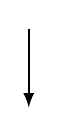
\begin{tikzpicture}
    \draw[-latex,thick](0,0) -- (0,-1); 
  \end{tikzpicture}
\end{center}

\begin{multicols}{2}
  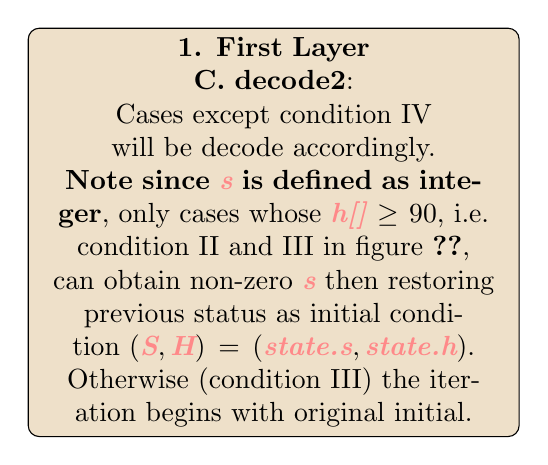
\begin{tikzpicture}
    \node [block]{
        \textbf{1. First Layer}\\
        \textbf{C. decode2}:\\
        Cases except condition \Romannum{4} will be decode accordingly.\\
        \textbf{Note since \para{s} is defined as integer}, only cases whose $\para{h[]}\geq 90$, i.e. condition \Romannum{2} and \Romannum{3} in figure \ref{fig:column}, can obtain non-zero \para{s} then restoring previous status as initial condition $(\para{S},\para{H})=(\para{state.s},\para{state.h})$. Otherwise (condition \Romannum{3}) the iteration begins with original initial.
      };
  \end{tikzpicture}
 \columnbreak
 \begin{minted}{cpp}
      else {
	int s = (h.x[] + HSHIFT/2.)/100.;
	state.h = h.x[] - 100.*s;
	state.s = s - 1;
      }

      if (state.s != complete)
	S = state.s, H = state.h;
    }
 \end{minted}
\end{multicols}

\begin{center}
  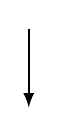
\begin{tikzpicture}
    \draw[-latex,thick](0,0) -- (0,-1); 
  \end{tikzpicture}
\end{center}
\newpage

\begin{multicols}{2}
  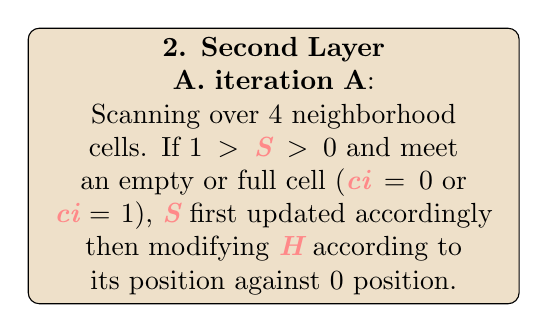
\begin{tikzpicture}
    \node [block]{
        \textbf{2. Second Layer}\\
        \textbf{A. iteration A}:\\
        Scanning over 4 neighborhood cells. If $1>\para{S}>0$ and meet an empty or full cell ($\para{ci}=0$ or $\para{ci}=1$), \para{S} first updated accordingly then modifying \para{H} according to its position against 0 position.
      };
  \end{tikzpicture}
 \columnbreak
 \begin{minted}{cpp}
    for (int i = 1; i <= 4; i++) {
      ci = i <= 2 ? c[i*j] : cs.x[(i - 2)*j];
      H += ci;

      if (S > 0. && S < 1.) {
	S = ci;
	if (ci <= 0. || ci >= 1.) {
	  H -= i*ci;
	  break;
	}
      }
 \end{minted}
\end{multicols}

\begin{center}
  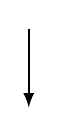
\begin{tikzpicture}
    \draw[-latex,thick](0,0) -- (0,-1); 
  \end{tikzpicture}
\end{center}

\begin{multicols}{2}
  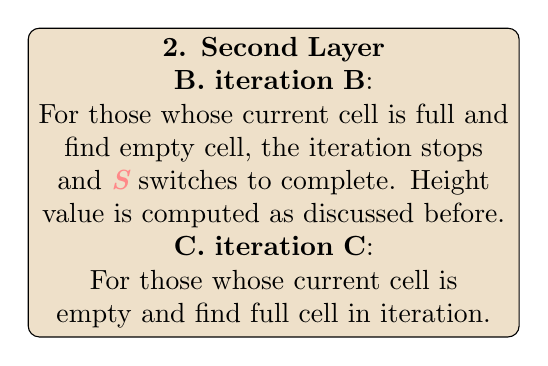
\begin{tikzpicture}
    \node [block]{
        \textbf{2. Second Layer}\\
        \textbf{B. iteration B}:\\
        For those whose current cell is full and find empty cell, the iteration stops and \para{S} switches to complete. Height value is computed as discussed before.\\
        \textbf{C. iteration C}:\\
        For those whose current cell is empty and find full cell in iteration.
      };
  \end{tikzpicture}
 \columnbreak
 \begin{minted}{cpp}
      else if (S >= 1. && ci <= 0.) {
	H = (H - 0.5)*j + (j == -1)*HSHIFT;
	S = complete;
	break;
      }
      else if (S <= 0. && ci >= 1.) {
	H = (i + 0.5 - H)*j + (j == 1)*HSHIFT;
	S = complete;
	break;
      }
 \end{minted}
\end{multicols}

\begin{center}
  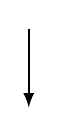
\begin{tikzpicture}
    \draw[-latex,thick](0,0) -- (0,-1); 
  \end{tikzpicture}
\end{center}

\begin{multicols}{2}
  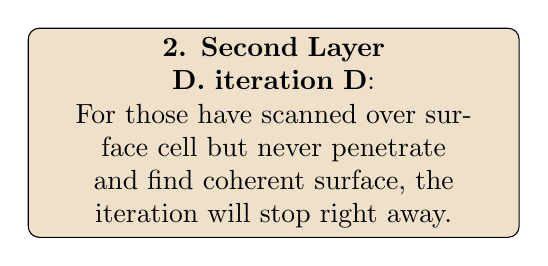
\begin{tikzpicture}
    \node [block]{
        \textbf{2. Second Layer}\\
        \textbf{D. iteration D}:\\
        For those have scanned over surface cell but never penetrate and find coherent surface, the iteration will stop right away.
      };
  \end{tikzpicture}
 \columnbreak
 \begin{minted}{cpp}
      else if (S == ci && modf(H, &a))
	break;
    }
 \end{minted}
\end{multicols}

\begin{center}
  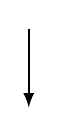
\begin{tikzpicture}
    \draw[-latex,thick](0,0) -- (0,-1); 
  \end{tikzpicture}
\end{center}

\begin{multicols}{2}
  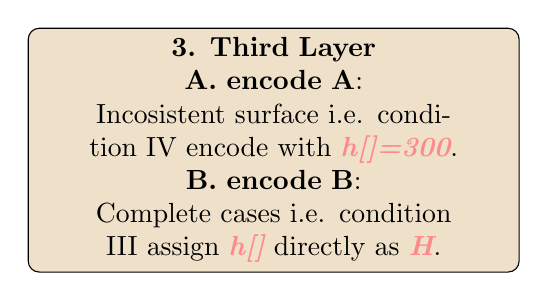
\begin{tikzpicture}
    \node [block]{
        \textbf{3. Third Layer}\\
        \textbf{A. encode A}:\\
        Incosistent surface i.e. condition \Romannum{4} encode with $\para{h[]=300}$.\\
        \textbf{B. encode B}:\\
        Complete cases i.e. condition \Romannum{3} assign \para{h[]} directly as \para{H}.
      };
  \end{tikzpicture}
 \columnbreak
 \begin{minted}{cpp}
    if (j == -1) {
      if (S != complete && ((c[] <= 0. || c[] >= 1.) || (S > 0. && S < 1.)))
	h.x[] = 300.; // inconsistent
      else if (S == complete)
	h.x[] = H;
 \end{minted}
\end{multicols}

\newpage

\begin{center}
  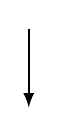
\begin{tikzpicture}
    \draw[-latex,thick](0,0) -- (0,-1); 
  \end{tikzpicture}
\end{center}

\begin{multicols}{2}
  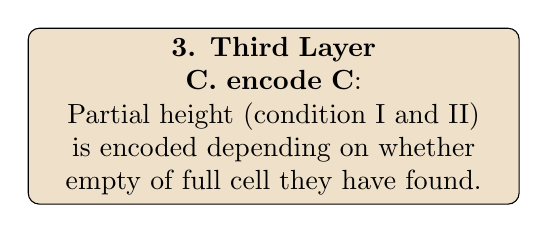
\begin{tikzpicture}
    \node [block]{
        \textbf{3. Third Layer}\\
        \textbf{C. encode C}:\\
        Partial height (condition \Romannum{1} and \Romannum{2}) is encoded depending on whether empty of full cell they have found.\\
      };
  \end{tikzpicture}
 \columnbreak
 \begin{minted}{cpp}
      else
	h.x[] = H + 100.*(1. + (S >= 1.));
    }
 \end{minted}
\end{multicols}

\begin{center}
  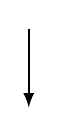
\begin{tikzpicture}
    \draw[-latex,thick](0,0) -- (0,-1); 
  \end{tikzpicture}
\end{center}

\begin{multicols}{2}
  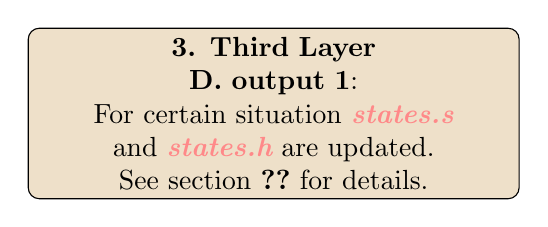
\begin{tikzpicture}
    \node [block]{
        \textbf{3. Third Layer}\\
        \textbf{D. output 1}:\\
        For certain situation \para{states.s} and \para{states.h} are updated. See section \ref{sec:thirdl} for details.\\
      };
  \end{tikzpicture}
 \columnbreak
 \begin{minted}{cpp}
    else { // j = 1
	  
      if (state.s != complete ||
	  (S == complete && fabs(height(H)) < fabs(height(state.h))))
	state.s = S, state.h = H;
    }
 \end{minted}
\end{multicols}

\begin{center}
  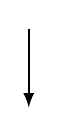
\begin{tikzpicture}
    \draw[-latex,thick](0,0) -- (0,-1); 
  \end{tikzpicture}
\end{center}

\begin{multicols}{2}
  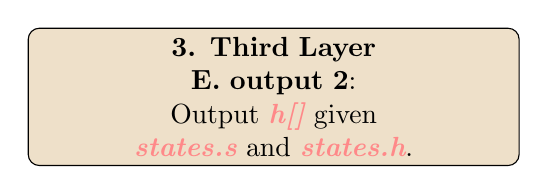
\begin{tikzpicture}
    \node [block]{
        \textbf{3. Third Layer}\\
        \textbf{E. output 2}:\\
        Output \para{h[]} given \para{states.s} and \para{states.h}.\\
      };
  \end{tikzpicture}
 \columnbreak
 \begin{minted}{cpp}
      if (state.s != complete)
	h.x[] = nodata;
      else
	h.x[] = (state.h > 1e10 ? nodata : state.h);
    }
  }
}
 \end{minted}
\end{multicols}

\subsection{\func{column\_propagation}}
Function \func{column\_propagation} serves as supplement of \func{half\_column} which allocates height value to those located within $5.5R$ from the 0 position but gain $nodata$ from \func{half\_column}. Take cell $G$ in figure \ref{fig:hvcomp} as an example, such cell is indeed valid and should be assigned with $-3.8$ as its height value. However, owing to failure of finding coherent surface in its four neighbors, the cell is actually assigned with $nodata$. \func{column\_propagation} is therefore built for tackling such issue.
\subsubsection{Parameters}
\begin{center}
  \begin{tabular}{|c|c|c|c|c|}
    \hline
    Name & Data type & Status & Option/Default & Representation (before/after)\\[0.5ex]
    \hline\hline
    \rowcolor{output}\para{h} & vector & \textbf{update} & compulsory & $\mathbf{h}$\\
    \hline
  \end{tabular}
\end{center}
\subsubsection{Worth Mentioning Details}
Similar to the process in \func{half\_column}, current function will iterate two neighbors in both directions and update height value base on spatial relation with the smallest height cell.
\subsubsection{Program Workflow}
\begin{multicols}{2}
  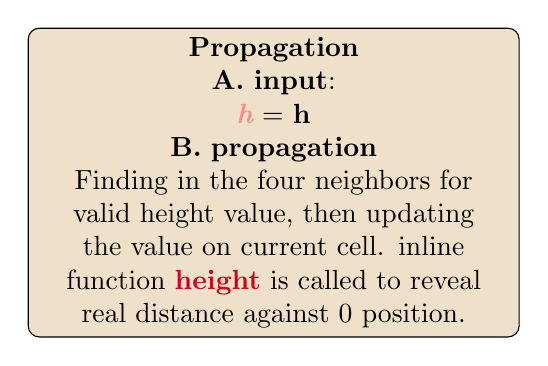
\begin{tikzpicture}
    \node [block]{
        \textbf{Propagation}\\
        \textbf{A. input}:\\
        \para{h} = $\mathbf{h}$\\
        \textbf{B. propagation}\\
        Finding in the four neighbors for valid height value, then updating the value on current cell. inline function \func{height} is called to reveal real distance against 0 position.
      };
  \end{tikzpicture}
 \columnbreak
 \begin{minted}{cpp}
static void column_propagation (vector h)
{
  foreach (serial) // not compatible with OpenMP
    for (int i = -2; i <= 2; i++)
      foreach_dimension()
	if (fabs(height(h.x[i])) <= 3.5 &&
	    fabs(height(h.x[i]) + i) < fabs(height(h.x[])))
	  h.x[] = h.x[i] + i;
}
 \end{minted} 
\end{multicols}

\subsection{\func{heights} for non-tree grid}
As introduced in section \ref{sec:config}, \func{heights} serves as a controller over \func{half\_column} and \func{column\_propagation} to assign height value to valid cells. The non-tree grid version is first introduced which shares the same construction with tree grid version.

\subsubsection{Parameters}
\begin{center}
  \begin{tabular}{|c|c|c|c|c|}
    \hline
    Name & Data type & Status & Option/Default & Representation (before/after)\\[0.5ex]
    \hline\hline
    \para{c} & scalar & unchanged & compulsory & color function $c$\\
    \hline
    \rowcolor{output}\para{h} & vector & \textbf{update} & compulsory & $\mathbf{h}$\\
    \hline
  \end{tabular}
\end{center}

\subsubsection{Worth Mentioning Details}
Since there are only two cells for the boundary in default settings, an additional vector \para{s} is create to meet the need for iterating $4$ cells in both direction. In particular, the value stored in position $[x_0,y_0]$ for \para{s} is
\begin{equation}\label{equ:translation}
    s.x[x_0,y_0] = c[x_0+2j,y_0]
\end{equation}
where \para{j} is the parameter implies the direction (see figure \ref{fig:funcconfig}). Notably, each components of \para{s} indicates value translation of corresponding direction.

\subsubsection{Program Workflow}
\begin{multicols}{2}
  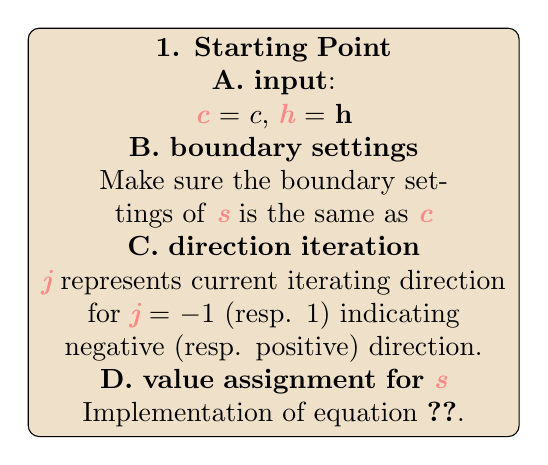
\begin{tikzpicture}
    \node [block]{
        \textbf{1. Starting Point}\\
        \textbf{A. input}:\\
        \para{c} = $c$, \para{h} = $\mathbf{h}$\\
        \textbf{B. boundary settings}\\
        Make sure the boundary settings of \para{s} is the same as \para{c}\\
        \textbf{C. direction iteration}\\
        \para{j} represents current iterating direction for \para{j} = $-1$ (resp. $1$) indicating negative (resp. positive) direction.\\
        \textbf{D. value assignment for \para{s}}\\
        Implementation of equation \ref{equ:translation}.
        
      };
  \end{tikzpicture}
 \columnbreak
 \begin{minted}{cpp}
#if !TREE
trace
void heights (scalar c, vector h)
{
  vector s[];
  foreach_dimension()
    for (int i = 0; i < nboundary; i++)
      s.x.boundary[i] = c.boundary[i];
  for (int j = -1; j <= 1; j += 2) {
    foreach()
      foreach_dimension()
        s.x[] = c[2*j];
 \end{minted} 
\end{multicols}

\begin{center}
  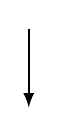
\begin{tikzpicture}
    \draw[-latex,thick](0,0) -- (0,-1); 
  \end{tikzpicture}
\end{center}

\begin{multicols}{2}
  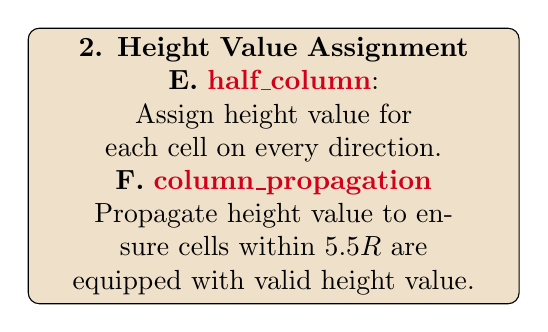
\begin{tikzpicture}
    \node [block]{
        \textbf{2. Height Value Assignment}\\
        \textbf{E. \func{half\_column}}:\\
        Assign height value for each cell on every direction.\\
        \textbf{F. \func{column\_propagation}}\\
        Propagate height value to ensure cells within $5.5R$ are equipped with valid height value.
      };
  \end{tikzpicture}
 \columnbreak
 \begin{minted}{cpp}
    foreach (overflow)
      half_column (point, c, h, s, j);
  }
  column_propagation (h);
}
 \end{minted} 
\end{multicols}
\printbibliography
\end{document}
